\chapter{Materiales y métodos} 

% ------------------------------------------------------------------------------------------------------------
% ------------------------------------------------------------------------------------------------------------

\section{Conjunto de datos disponibles}

% ------------------------------------------------------------------------------------------------------------

%\subsection{Radiografías panorámicas maxilofaciales}

Disponemos de un conjunto de datos compuesto por radiografías panorámicas maxilofaciales de individuos de 
diversos países y continentes (véase en la tabla \ref{tab:instituciones_fuente_dataset}), obtenidas con
distintos modelos de máquinas de rayos X
\footnote{
    Los modelos empleados fueron: \textit{Planmeca Promax Digital Panoramic}; \textit{Sirona ORTHOPHOS-XG}, 
    \textit{ORTHOPHOS-DS}, y \textit{SIDEXIS}. Las constantes radiológicas usadas fueron de 66 a a 70 kV, 7 a 
    11 mA, y 15 s.
}. 
Este conjunto de datos ha sido sido proporcionados por Panacea Cooperative Research, empresa \textit{spin-off} 
de la Universidad de Granada.  

\begin{table}[h]
\begin{tabular}{@{}clc@{}}
\toprule
País                                                            & Instituciones                                                                                                                                                            & Nº de ejemplos \\ \midrule
\begin{tabular}[c]{@{}c@{}}Bosnia y \\ Herzegovina\end{tabular} & Universidad de Sarajevo                                                                                                                                                  & 882            \\ \hline
Botsuana                                                        & \begin{tabular}[c]{@{}l@{}}Dos clínicas dentales privadas en \\ Garobone\end{tabular}                                                                                    & 1242           \\ \hline
Chile                                                           & \begin{tabular}[c]{@{}l@{}}Dos clínicas dentales privadas en \\ Santiago y Rancagua\end{tabular}                                                                         & 1016           \\ \hline
\begin{tabular}[c]{@{}c@{}}República \\ Dominicana\end{tabular} & \begin{tabular}[c]{@{}l@{}}Tres clínicas dentales privadas en \\ Santo Domingo, La Vega y Santiago\end{tabular}                                                          & 541            \\ \hline
Japón                                                           & \begin{tabular}[c]{@{}l@{}}Department of Forensic Sciences, \\ Iwate Medical University, Iwate\end{tabular}                                                              & 1045           \\ \hline
Corea                                                           & Catholic University of Korea, Seoul                                                                                                                                      & 500            \\ \hline
Malasia                                                         & \begin{tabular}[c]{@{}l@{}}Faculty of Dentistry Universiti Teknologi \\ MARA Selangor Branch, Selangor\end{tabular}                                                      & 667            \\ \hline
Turquía                                                         & \begin{tabular}[c]{@{}l@{}}Department of Dentomaxillofacial \\ Radiology, Baskent University, Turkey\end{tabular}                                                        & 2323           \\ \hline
Uganda                                                          & \begin{tabular}[c]{@{}l@{}}Department of Dental Morphology with \\ the Université Claude Bernard Lyon 1, \\Faculté d’odontologie, Lyon\end{tabular}                      & 283            \\ \hline
Italia                                                          & \begin{tabular}[c]{@{}l@{}}Department of Surgical Sciences, \\ University of Cagliari\end{tabular}                                                                       & 173            \\ \hline
Kosovo                                                          & \begin{tabular}[c]{@{}l@{}}University Dentistry Clinical Center, \\ Pristina\end{tabular}                                                                                & 1397           \\ \hline
Líbano                                                          & Clínica dental privada en Beirut                                                                                                                                         & 690            \\ \bottomrule
\end{tabular}
\caption[
    Instituciones participantes en la recolección de datos e imágenes
]{   
    Lista de instituciones participantes en la recolección de los datos e imágenes dentales utilizados en el 
    trabajo.
}
\label{tab:instituciones_fuente_dataset}
\end{table}

Este \textit{dataset} incluye:

\begin{itemize}

    \item datos tabulares (en formato CSV), donde cada fila representa un ejemplo (un individuo), con los 
    siguientes campos: un identificador único, sexo del individuo, edad del individuo y ``muestra'' 
    (clasificación según el origen geográfico de la radiografía), e

    \item imágenes bidimensionales de radiografías panorámicas maxilofaciales, con una imagen asociada 
    a cada individuo y se identifica mediante su ID único. 

\end{itemize}

Se proporcionan los datos ya preprocesados, por lo que no es necesario realizar tareas adicionales de limpieza 
o transformación previa antes de su análisis.

Se ignora el campo de ``muestra'', dado que se trata de una asignación
sesgada y no representa necesariamente una clasificación fiable del origen poblacional de los individuos.
Por tanto, este campo no se emplea en el análisis ni en el entrenamiento de los modelos, centrándose 
exclusivamente en las variables de edad, sexo e imagen.

En el \textit{dataset} hay un total de 10.739 ejemplos, de los que 5.756 son de individuos de sexo femenino 
y 4.983 de sexo masculino. 
Las edades mínima y máxima son 14 y 26 años, respectivamente, y la media son 19,13 años.
En la Figura \ref{fig:histogram_ages} se observa que el número de ejemplos por edad se mantiene relativamente 
constante desde los 14 hasta los 21 años, a partir de los cuales disminuye progresivamente, con una 
representación notablemente menor en los grupos de 24, 25 y 26 años.
 
\begin{figure}[h]
    \centering
    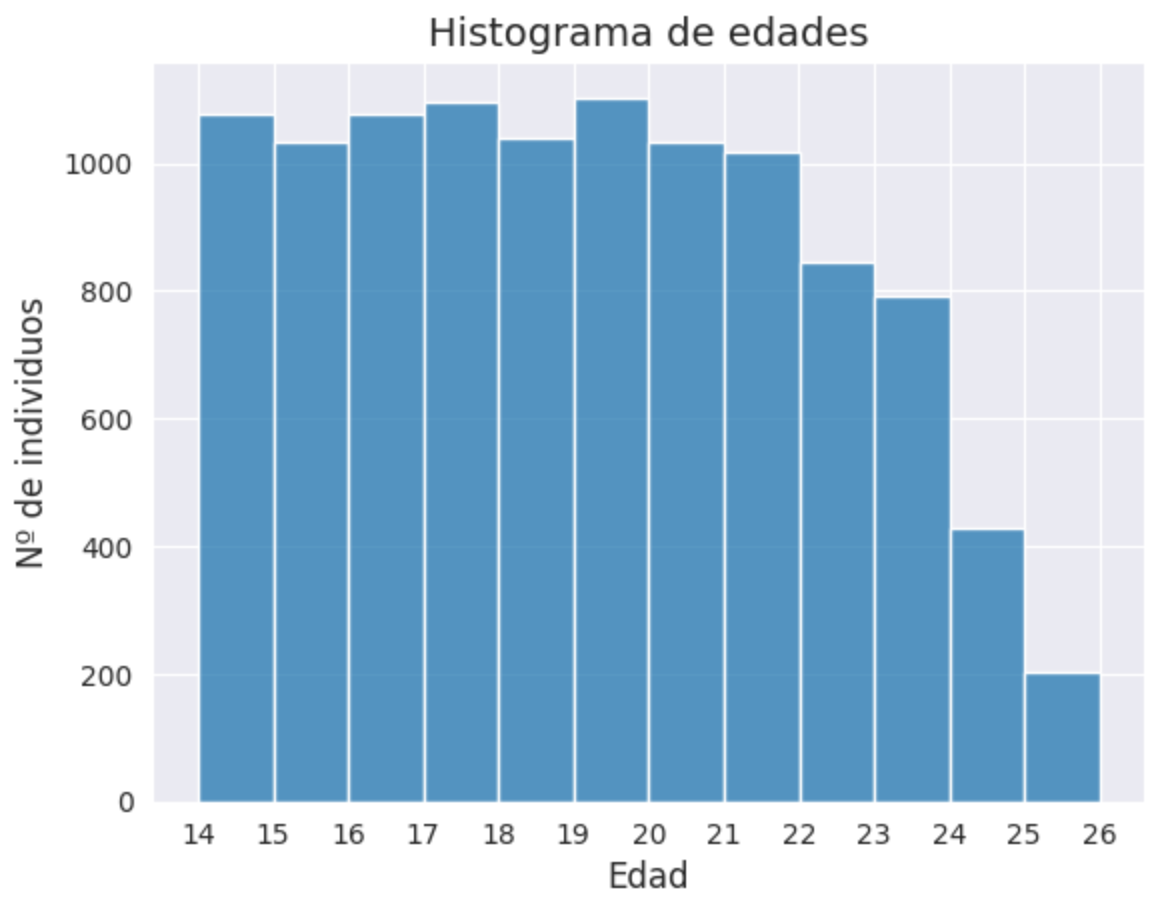
\includegraphics[width=0.7\textwidth]{capitulos/cap_04/imagenes/histogram_ages.png}
    \caption[
        Distribución de edad de los individuos del conjunto de datos disponible.
    ]{
        Distribución de edad de los individuos del conjunto de datos disponible. Elaboración propia.
    } 
    \label{fig:histogram_ages}
\end{figure}

En la Figura \ref{fig:kde_and_boxplot_ages_sex} podemos comprobar cómo en términos relativos la distribución 
de edad por sexo es muy similar, compartiendo ambas prácticamente el mismo rango de edades y patrones de 
dispersión, sin observarse diferencias sustanciales en la mediana ni en la forma general de las 
distribuciones.

\begin{figure}[h]
    \centering
    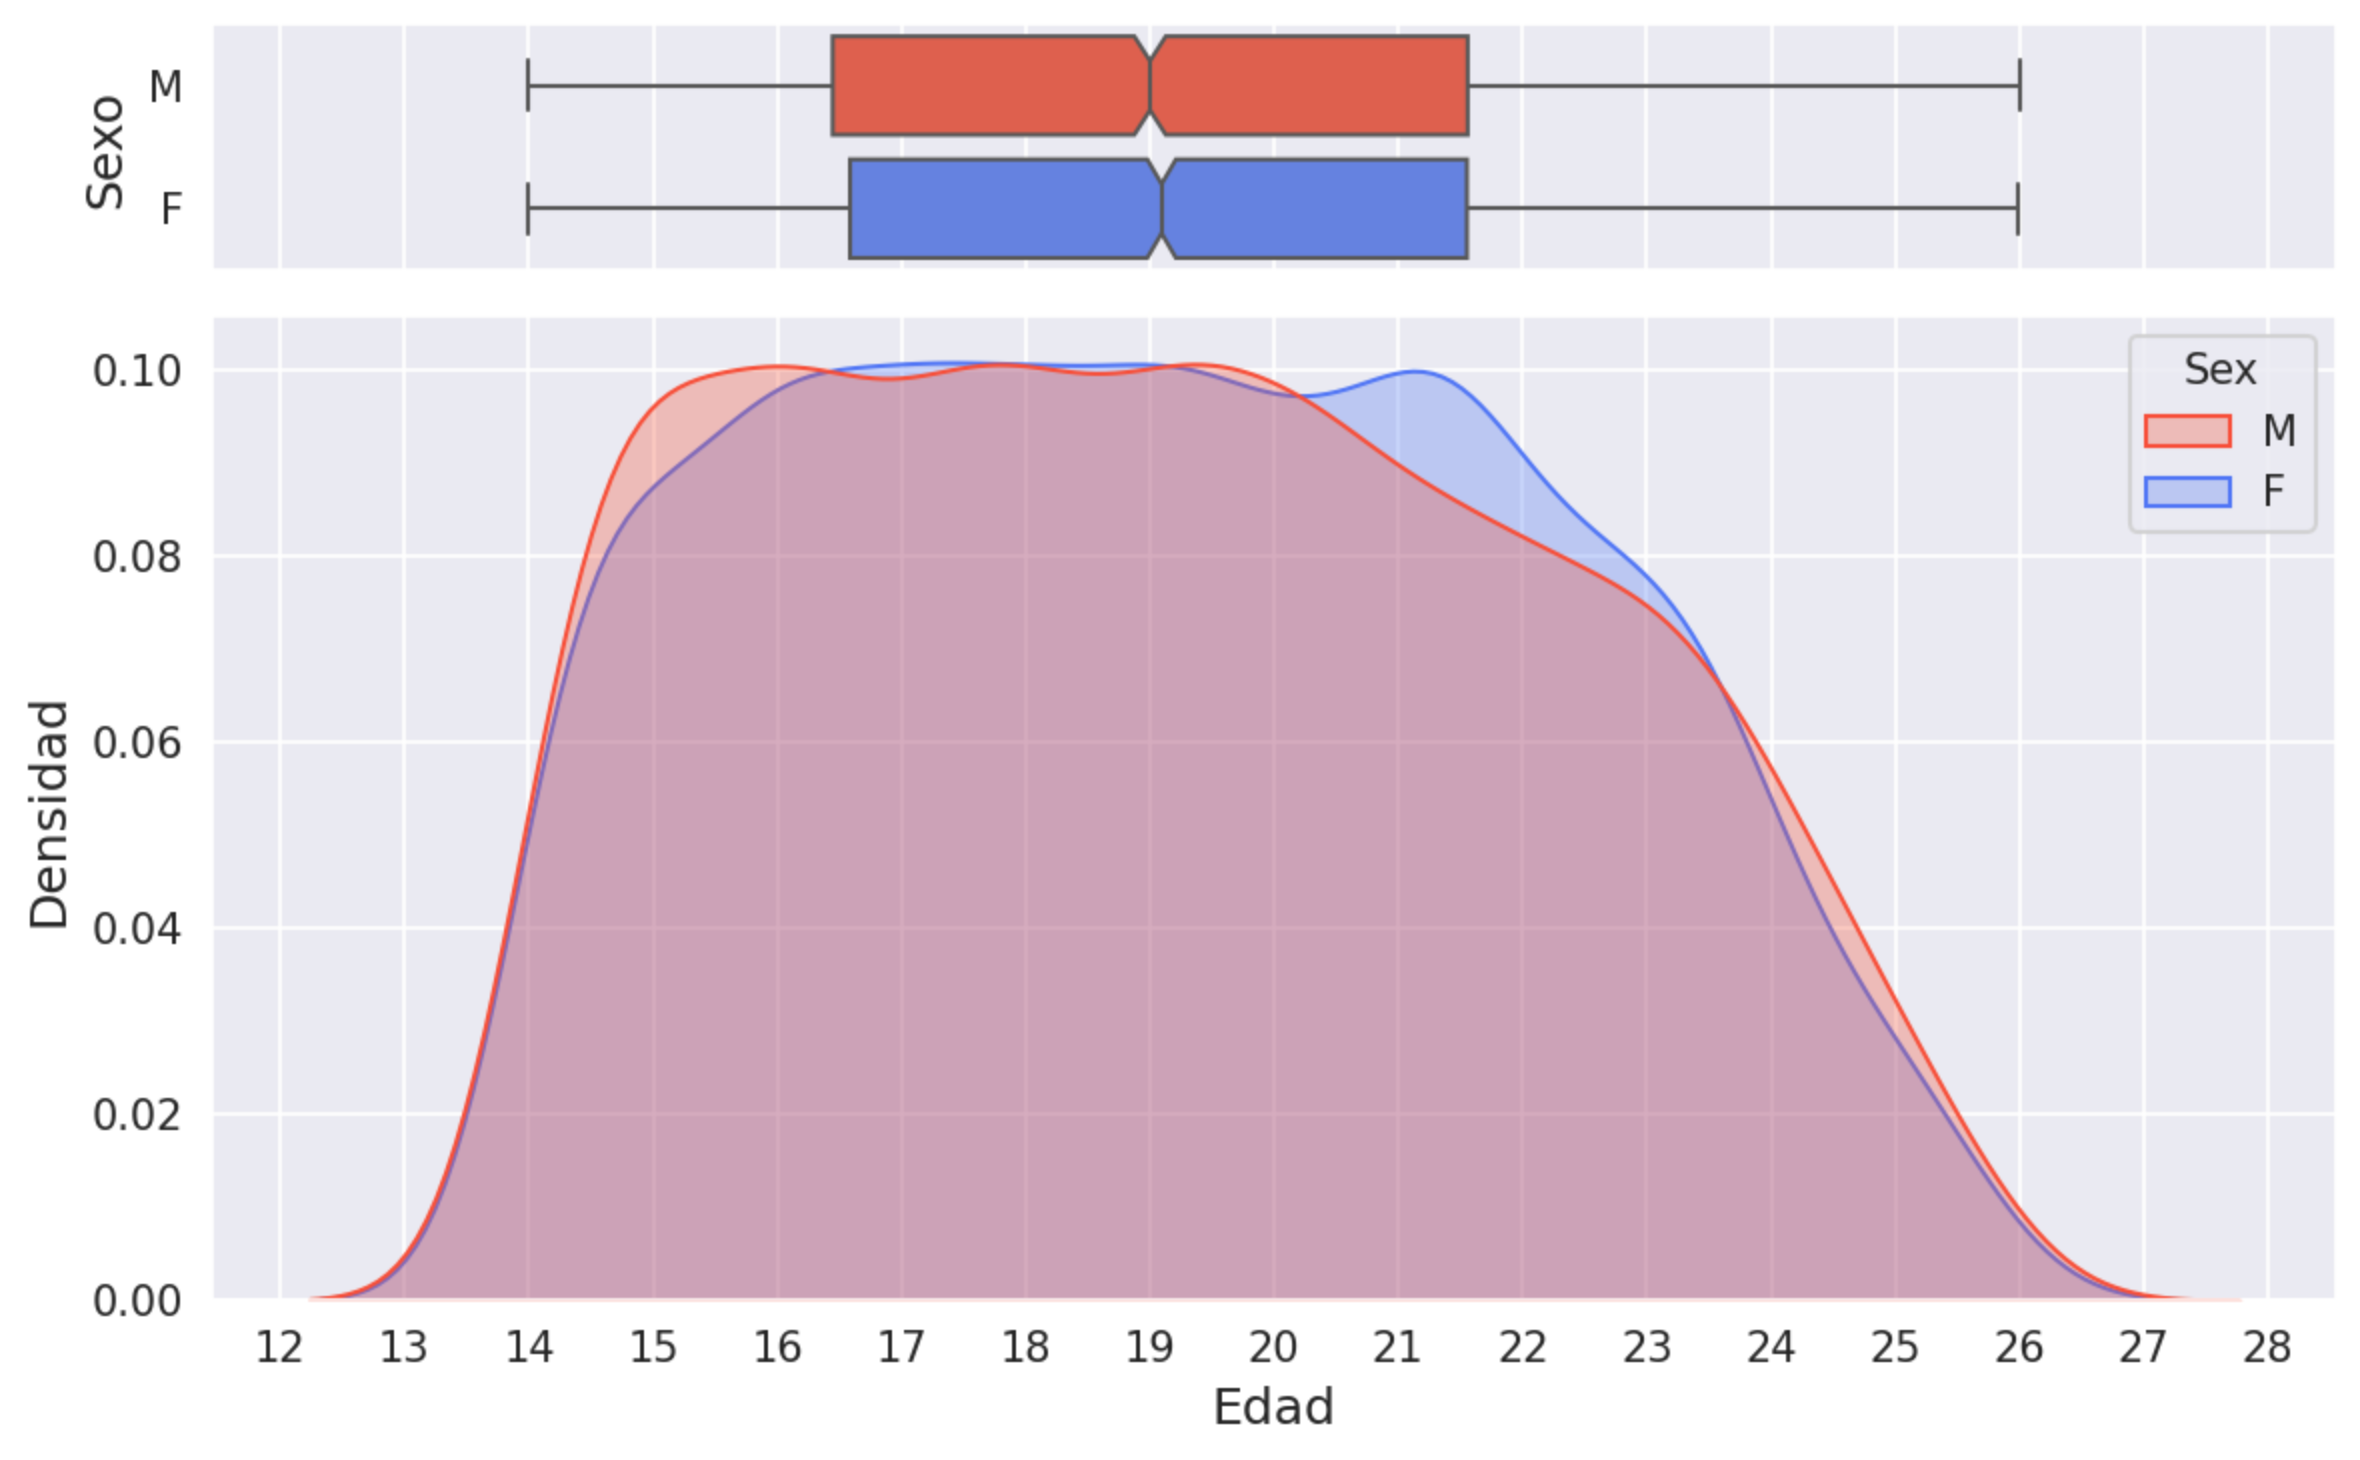
\includegraphics[width=\textwidth]{capitulos/cap_04/imagenes/kdeplot_ages.png}
    \caption[
        Distribución de edad por sexo de los individuos del conjunto de datos disponible.
    ]{
        Distribución de edad por sexo de los individuos del conjunto de datos disponible. Elaboración propia.
    } 
    \label{fig:kde_and_boxplot_ages_sex}
\end{figure}

En conclusión, el dataset presenta en general un buen balance entre clases y edades, lo que permite un 
análisis representativo de la población incluida. No obstante, será necesario examinar con mayor detalle la 
infrarepresentación de los grupos de mayor edad, especialmente a partir de los 22 años, para evaluar su 
posible impacto en el rendimiento y generalización de los modelos entrenados.

Se proporcionan los datos ya divididos en \textit{train} ---con un 80\% de los individuos--- y \textit{test}
---con el 20\% restante---, con la intención de que puedan ser utilizados para entrenar y evaluar modelos de 
predicción. En la Figura \ref{fig:kde_ages_train_test} se puede observar cómo existe una distribución 
edad-sexo similar en los datos de ambos subconjuntos, por lo que se puede asumir que la partición respeta la 
representatividad de la población original, favoreciendo una evaluación más realista del rendimiento de los 
modelos en datos no vistos.

\begin{figure}[h]
        \centering

        \begin{subfigure}[b]{0.47\textwidth}
            \centering
            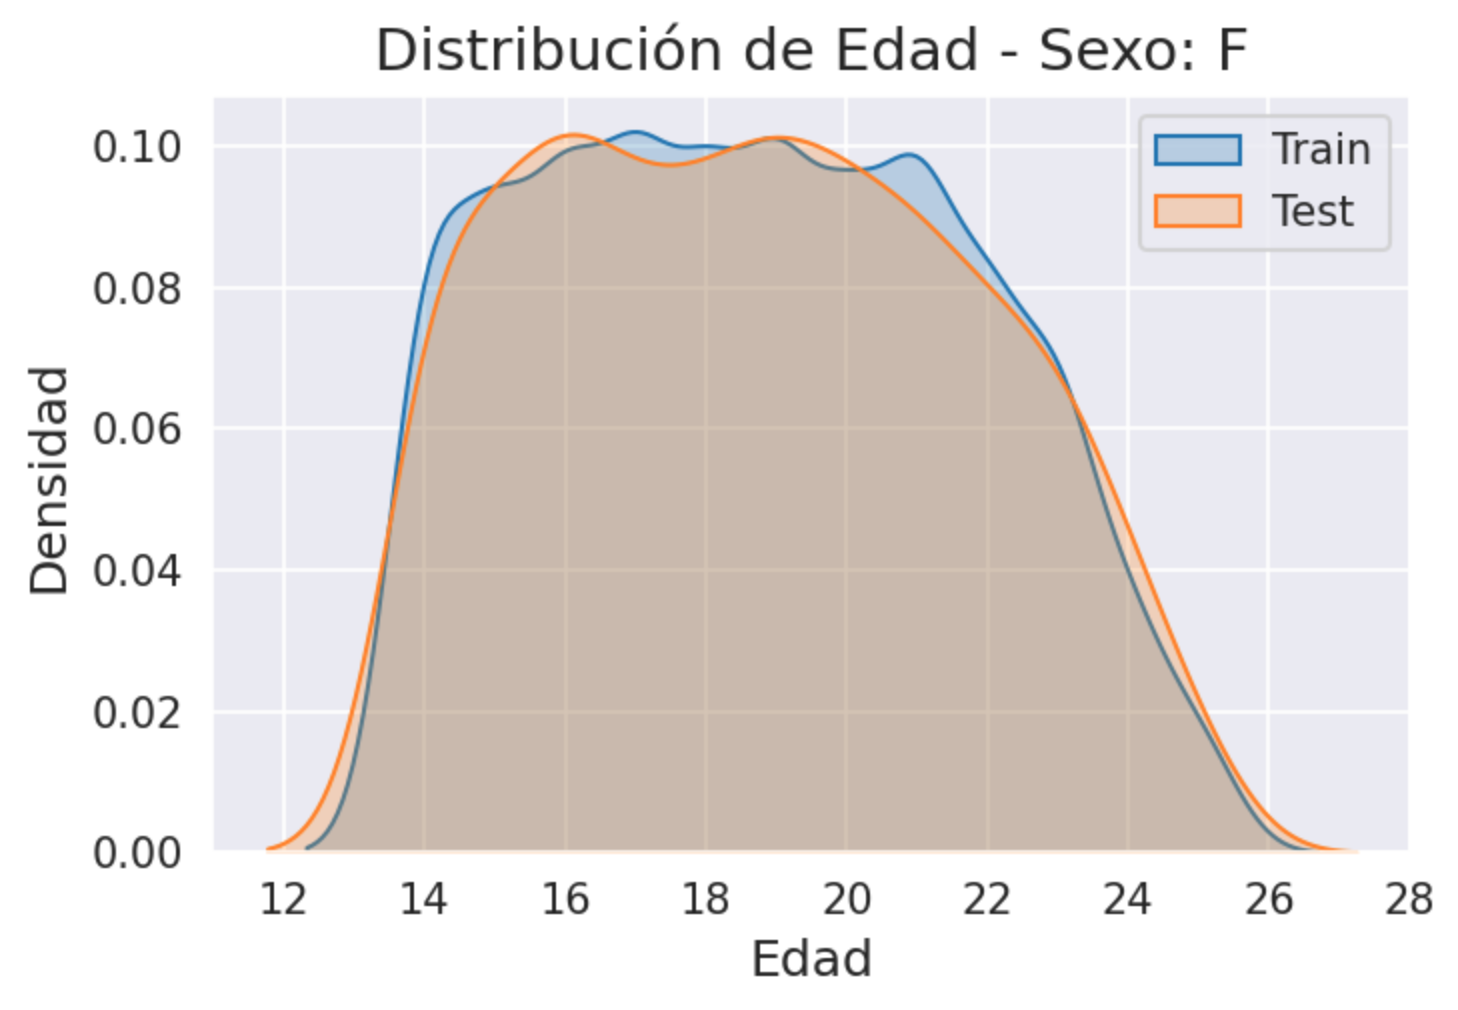
\includegraphics[width=\textwidth]{capitulos/cap_04/imagenes/kde_ages_F.png}
            \caption{Distribución de edad de individuos de sexo femenino.}
            \label{fig:kde_ages_F}
        \end{subfigure}
        \hfill
        \begin{subfigure}[b]{0.47\textwidth}
            \centering
            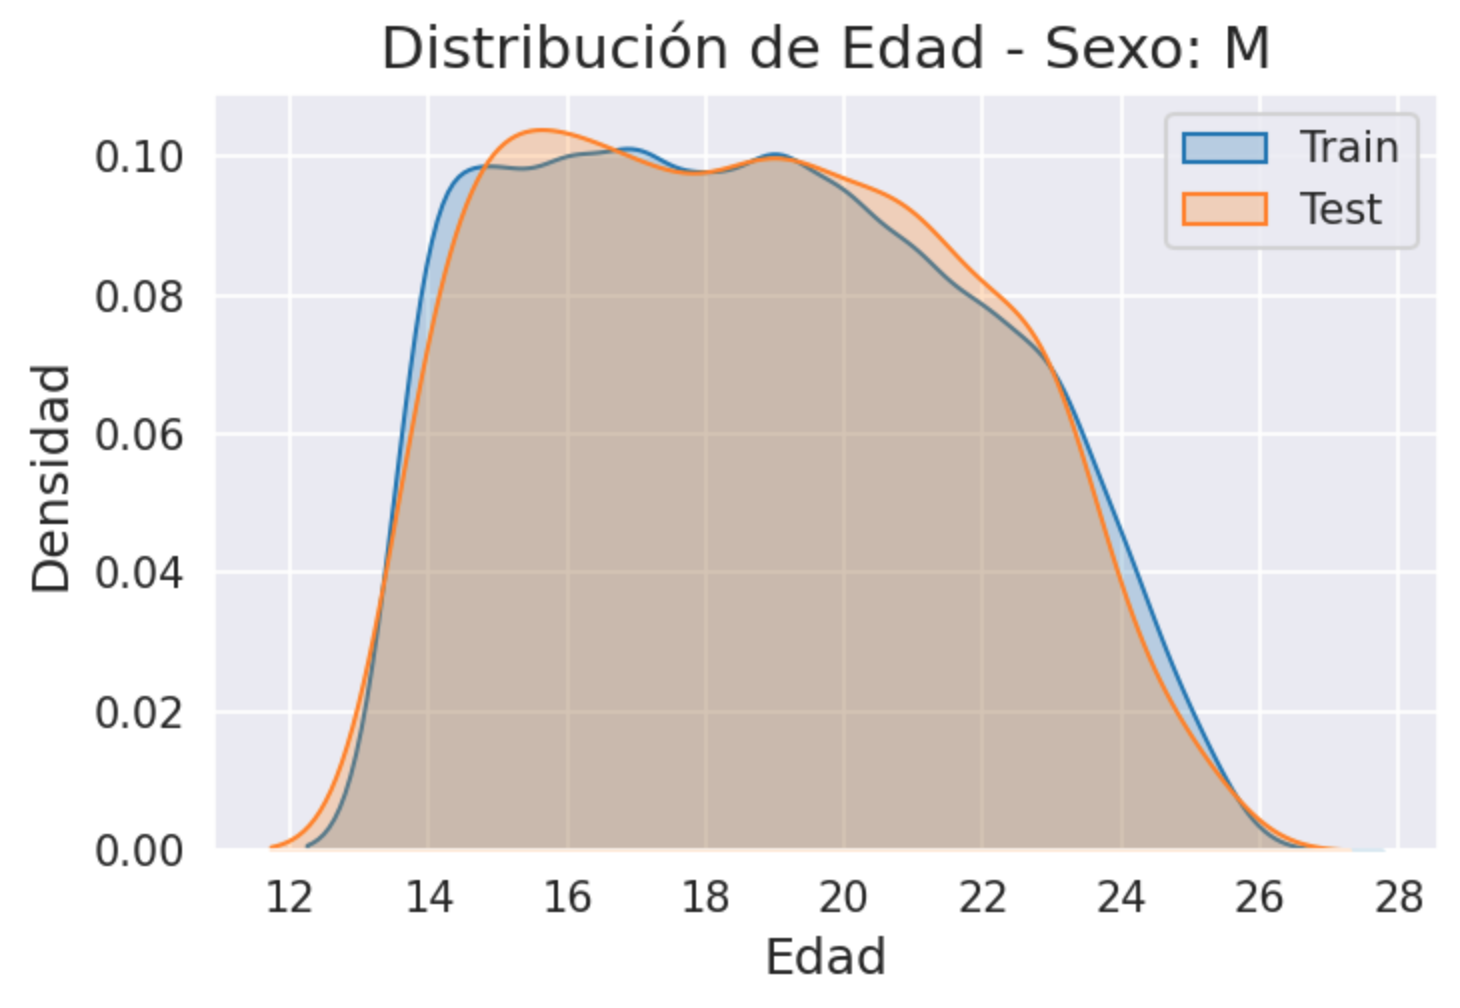
\includegraphics[width=\textwidth]{capitulos/cap_04/imagenes/kde_ages_M.png}
            \caption{Distribución de edad de individuos de sexo masculino.}
            \label{fig:kde_ages_M}
        \end{subfigure}

        \caption[
            Distribución de edad de los individuos del conjunto de datos disponible por sexo.
        ]{
            Distribución de edad de los individuos del conjunto de datos disponible por sexo. 
            Elaboración propia.
        }
        \label{fig:kde_ages_train_test}
    \end{figure}


% ------------------------------------------------------------------------------------------------------------
% ------------------------------------------------------------------------------------------------------------

\section{Métodos propuestos}

\subsection{Arquitectura empleada}

El primer problema propuesto es el de estimación de edad. Partiremos de un planteamiento muy simple: imágenes 
bidimensionales de las radiografías panóramicas maxilofaciales como entrada, y estimación de edad a la salida.
No incorporaremos el sexo del individuo en esta primera aproximación, si bien se explorará en el Anexo X. 
\todo{¿Finalmente incluimos o no el sexo el sexo del individuo?}

Como modelo, empleamos una CNN, dado su buen desempeño en tareas de visión por computador. Específicamente,
implementamos la arquitectura ResNeXt50 \cite{xie2017}, utilizando un modelo entrenado con el \textit{dataset} 
ImageNet
\footnote{
    El dataset Imagenet contiene 1.000 clases de objetos. Estas clases abarcan una
    amplia variedad de categorías, como animales (\textit{tiger}, \textit{koala}, \textit{zebra}, ...), 
    vehículos (\textit{ambulance}, \textit{airliner}, \textit{mountain bike}, ...), alimentos 
    (\textit{strawberry}, \textit{pizza}, \textit{bagel}, ...), entre otras. 
}
\cite{deng2009} como punto de partida. Este modelo preentrenado es accesible a través de Pytorch. 

Aunque ResNeXt50 fuera diseñado originalmente para un problema de clasificación de imágenes y entrenado con
un dominio distinto al de nuestro problema, su adaptación a una tarea de estimación de edad es sencilla: 
reemplazar su cabecera de clasificación por una de regresión. Además, el uso de peso preentrenados proporciona
una inicialización más robusta que el entrenamiento desde cero, ya que el modelo ya ha aprendido filtros 
genéricos para detectar características visuales básicas, como bordes o texturas.



\subsection{Entrenamiento}



\subsection{\textit{Split conformal regression}}


\subsection{Regresión cuantílica}


\subsection{\textit{Conformalized Quantile Regression}}


% ------------------------------------------------------------------------------------------------------------

\section{}





%Se suele determinar tamaños de lotes que sean potencias de dos, en el rango de 16 a 256 \cite{goodfellow2016}. 

% Una estrategia recomendada consiste en:

% \begin{enumerate}

%     \item Entrenar inicialmente solo el nuevo head (la capa o capas finales añadidas para la tarea específica) 
%     durante una época con una tasa de aprendizaje (learning rate) alta, manteniendo el resto de los parámetros 
%     del modelo congelados (sin actualizar).

%     \item Luego, realizar un entrenamiento adicional de todo el modelo (incluyendo las capas preentrenadas) 
%     con una tasa de aprendizaje más baja, permitiendo un ajuste fino (fine-tuning) de todos los parámetros.

% \end{enumerate}